% !TEX root = main.tex
%
% Introduction
%
Various extensions of language models for handling infinite alphabets have been proposed.
%words carrying data values in an infinite domain (e.g. integers) e.g. data processing
Some automata 
\reviews{1) and grammar with storage?}
with memory extensions
allow restricted storage and comparison of input symbols
%and correspond with logics,
(see~\cite{Segoufin06csl} for a survey)
\florent{register: skip refs and details, add Mikolaj recent}
using pebbles for marking positions~\cite{NevenSchwentickVianu04FSMinfinite},
registers~\cite{KaminskiFrancez94},
or %computations in 2 steps
the possibility to compute on subsequences
with the same attribute values~\cite{Bojanczyk11FO2}. % data words automata.
%
%for the and verification of infinite state systems
%(model checkers: alphabet = long bit-vectors)
%...For the representation of  in model checking, verification and
%
The automata at the core of model checkers
compute on input symbols represented by large bitvectors~\cite{Vardi07ciaa} %\cite{BaierKatoen08MC}
(sets of assignments of Boolean variables) %propositional variables)
and, in practice,  %implementation
each transition accepts a set of such symbols (instead of an individual symbol),
represented by Boolean Formulas or Binary Decision Diagrams.
%
Following a similar idea, % and generalizing,
in symbolic automata (\SA)~\cite{Veanes12symbolic,dAntoniVeanes17CAV,dAntoni21CACM},
transitions are guarded by predicates over infinite  domains.
With appropriate closure conditions on the sets of such predicates, % (alphabet theories),
all the good properties enjoyed over finite alphabets are preserved.

Other extensions of language models  %(automata and grammars)
help in dealing with non-determinism by computing weight values... associated to input..
*** In the context of parsing for instance, associating one weight to every grammar's derivation
permits to rank \emph{abstract syntax trees} -- AST, 
hence to select a best one (or $n$ bests) when using am ambiguous grammar, 
%This is roughly the principle of \emph{weighted parsing} approaches
\florent{introduce pb "weighted parsing" and ref.\cite{MorbitzVogler19weighted-parsing}.} 
%\reviews{1) jump from automata to grammars is uneasy and not really necessary}
% for which there may exist several derivations yielding one input word.
\florent{revise}
*** For verification, ... quantitative reasoning about programs
%
In \emph{weighted language models}~\cite{Goodman99SemiringParsing,Nederhof03weightedParsing,MorbitzVogler19weighted-parsing},
like \eg probabilistic context-free grammars % (CFG),
and weighted automata (\WA) \cite{Droste09handbook},
a weight is associated to each transition rule, % production rule
and the rule's weights can be combined with an
associative product operator~$\otimes$ to yield the weight of an AST.
\reviews{1) AST for grammar, run for WA}
A second operator~$\oplus$
is moreover used to resolve the ambiguity raised by the existence
of several (in general exponentially many) AST
associated to a given input word.
Typically, $\oplus$  selects the best of two weight values.
%Intuitively,~$\oplus$ selects, or ranking, the syntax trees.
The weight domain, equipped with these two operators is typically 
a \emph{semiring} %$\Semiring$
where $\oplus$ can be extended to infinite sums,
%\cite{Eilenberg74automata}
such as the Viterbi semiring and the tropical min-plus algebra% % see Figure~\ref{fig:semirings}.
%of domain $\mathbb{R}^+ \cup \{ +\infty\}$,
%where $\oplus$ is min and $\otimes$ is plus .
%by ranking
%making the weight domain a semiring.
%Some efficient specialized parsing algorithms~\cite{Huang05kbest} have been proposed in this context
%% models represented as hypergraphs \cite{Huang05kbest}
%in order to compute the $n$ best syntax trees of a given input word without having to enumerate them all.
%Generally based on dynamic programming, these algorithms rely on
%additional algebraic properties of~$\Semiring$.
%-- see \eg~\cite{Huang05kbest} for some NLP applications.
%The extraction of $n$ best list is useful
%the problem: quantitative parsing or symbolic parsing
%of parsing of words over infinite input alphabet.

In this paper, we present results for 
\emph{symbolic weighted} finite states language models (\swM) extensions
generalizing the Boolean guards of~\SA %in transitions
to functions into an arbitrary semiring, 
and generalizing also~\WA, by handling infinite alphabets (Figure~\ref{fig:hierarchy}).
...
\reviews{cite \cite{Herrmann16dlt,Herrmann20phd}}
%
In short, a transition rule $q \xrightarrow{\phi} q'$, from state $q$ to $q'$,
%\florent{c'est un résumé de la Fig. \ref{fig:hierarchy}}
%input symbols are variables, %(parameters)
is labeled by a function~$\phi$ associating to every input symbol $a$ a weight value $\phi(a)$
in a semiring $\Semiring$.

\begin{figure}
\centering
\begin{tikzpicture}
\node (SWADS) at (3.0,5.0) {%
  \(
  \begin{array}{c}
  \mathsf{SWADS}\,\mbox{\cite{Herrmann16dlt,Herrmann20phd}}
  \end{array}
  \)
};
%
\node (SWA) at (0,3.4) {%
  \(
  \begin{array}{c}
  \mathsf{SWA}: \Sigma_{\mathsf{inf}}^* \to \mathbb{S}\\
  q \xrightarrow{\phi} q', \phi : \Sigma_\mathsf{inf} \to \mathbb{S}
  \end{array}
  \)
};
%
\node (WA) at (-1.8,1.7) {%
  \(
  \begin{array}{c}
  \mathsf{WA}\,\mbox{\cite{Droste09handbook}}: \Sigma_{\mathsf{fin}}^* \to \mathbb{S}\\
  q \xrightarrow{a, w} q', a \in \Sigma_\mathsf{fin}, w \in \mathbb{S}
  \end{array}
  \)
};
%
\node (SA) at (1.8,1.7) {%8
  \(
  \begin{array}{c}
  \mathsf{SA}\,\mbox{\cite{Veanes12symbolic,dAntoni21CACM}}: \Sigma_{\mathsf{inf}}^* \to \mathbb{B}\\
  q \xrightarrow{\phi} q', \phi : \Sigma_\mathsf{inf} \to \mathbb{B}
  \end{array}
  \)
};
%
\node (NFA) at (0,0) {%
  \(
  \begin{array}{c}
  \mathsf{FA} : \Sigma_{\mathsf{fin}}^* \to \mathbb{B}\\
  q \xrightarrow{a} q', a \in \Sigma_\mathsf{fin}
  \end{array}
  \)
};
%
\node (VPA) at (5.6,0) {%
  \(
  \mathsf{VPA}\,\mbox{\cite{AlurMadhusudan09nested}}
  \)
};
%
\node (WVPA) at (4.6,1.7) {%
  \(
  \mathsf{WVPA}\,\mbox{\cite{Mathissen08weighted,Caralp12VPAmult}}
  \)
};
%
\node (SVPA) at (6.6,1.7) {%
  \(
  \mathsf{SVPA}\,\mbox{\cite{dAntonyAlur14SVPDA}}
  \)
};
%
\node (SWVPA) at (5.6,3.4) {%
  \(
  \mathsf{SWVPA}
  \)
};
%
\draw[->] (NFA)--(WA);
\draw[->] (NFA)--(SA);
\draw[->] (WA)--(SWA);
\draw[->] (SA)--(SWA);
\draw[->] (SWA)--(SWADS);
\draw[->] (VPA)--(WVPA);
\draw[->] (VPA)--(SVPA);
\draw[->] (WVPA)--(SWVPA);
\draw[->] (SVPA)--(SWVPA);
\draw[->] (SWVPA)--(SWADS);
%\begin{array}{c} \mathsf{NFA} : \Sigma^* \to \mathbb{B} \end{array}
\end{tikzpicture}
\caption{Classes of Symbolic/Weighted Automata.
Here, $\Sigma_\mathsf{fin}$ and $\Sigma_\mathsf{inf}$ denote finite/countable alphabets,
$\mathbb{B}$  the Boolean algebra,
$\mathbb{S}$ a commutative semiring.
$q \xrightarrow{\dots} q'$ is a transition between states $q$ and $q'$.}
\label{fig:hierarchy}
\end{figure}
%
%This approach is close to the case of
%Symbolic Automata (SA)~\cite{dAntoniVeanes17CAV,dAntoni21CACM},
%except that the domain for weight values is not restricted to be Boolean,
%like for the guards in the rules of SA,
%but can be an arbitrary commutative semiring (assuming some restrictions).

%The framework relies on several language models:
The models studied are: 
symbolic-weighted automata (\SWA),
transducers (\SWT), and pushdown automata
with a visibility restriction~\cite{AlurMadhusudan09nested} (\SWVPA).
A \SWT defines a distance $T(s, t)$ between finite words $s$ and $t$
over infinite alphabets. % following~\cite{Mohri03ijfcs}.
%\wrt an edit distance
A  \SWVPA operates sequentially on \emph{nested words}~\cite{AlurMadhusudan09nested},
structured with markup symbols (parentheses) and describing linearizations of trees.
A \SWVPA $A$ associates a weight value $A(t)$ % \in \Semiring$
to a given nested word $t$, which is itsef the linearization of a weighted AST. %representing a parse tree.

\SWA and \SWVPA are both particular cases of \cite{Herrmann16dlt,Herrmann20phd}, 
with special data storage types...
\florent{Both WA and SA generalized by \cite{Herrmann16dlt,Herrmann20phd}...}

THE RESULTS/CONTRIBUTIONS of this paper are:
\florent{revise: main results = 3 theorems}
%\reviews{1) not $i$! see response.txt}
%($i$)~the introduction of automata, \SWA, transducers, \SWT (Section~\ref{section:SWA}),
%and visibly pushdown automata \SWVPA (Section~\ref{sec:SWVPA}),
%generalizing the corresponding classes of symbolic and weighted models,
%for the weighted computation on (nested) words over infinite alphabets;
($i$)~a construction %Bar-Hillel Perles Shamir 
for computing a \SWT-defined distance between an \SWA language and a word (Section~\ref{section:SWA}), 
($ii$)~closure results for \SWVPA (Section~\ref{sec:SWVPA}), 
($iii$)~a polynomial best-search algorithm for \SWVPA, %(Section~\ref{sec:best})
% a framework for parsing over infinite alphabets,
%
Moreover, we detail 
($iv$)~an application to the problem of weighted parsing over infinite input alphabets 
(\emph{SW-parsing}, Section~\ref{sec:parsing}), 
based on the above models integrated in a uniform framework, with in particular:
($iv.a$)~the \SWT-based definition of generic edit distances between input and output (yield) words,
and ($iv.b$)~the use, for technical convenience, of nested words, and \SWVPA,
instead of syntax trees and grammars. %(\S~\ref{sec:trees}).

... These results should also apply in the context of the quantitive verification of programs...

***
Parsing is the problem of structuring a linear representation
(a finite word) according to a language model. % (a formal grammar). % natural language, programming language,
%
Most of the context-free parsing approaches~\cite{GruneJacobs08parsing}
assume a finite and reasonably small input alphabet. %models and algorithms
Such a restriction makes perfect sense in the context of
NLP tasks such as constituency parsing, 
compilers or interpreters for programming languages.
Considering large or infinite alphabets can however be of
practical interest when dealing with large characters encodings such as UTF-16~\cite{dAntoni21CACM},
\florent{applis à la Fossacs chez Veanes et al?}
% processing strings in \eg for vulnerability detection in Web-applications~\cite{dAntoni21CACM},
%
analysis of data streams, serialization of structured documents~\cite{Segoufin06csl,NevenSchwentickVianu04FSMinfinite},
or processing timed execution traces~\cite{Bouyer03algebraic}.
% algebraic definition of a class of data languages
% (notion of monoid recognizability, based on registers, comparable to Bojancszik et al. data words)

The latter case is related to a motivation  of  the present work: \florent{idem}
automated music transcription. Representations that capture  music performances
are essentially linear:
audio files or the widely used
MIDI format~\cite{Selfridge-Field97beyondMIDI}. %\cite{MIDIfile}.
Such representations ignore the hierarchical structures that frame the
conception of music, at least in the Western area. These structures, on the other hand,
are present, either explicitly  or implicitly,
in Common Western Music Notation~\cite{Gould11Notation}:
%in music notation~\cite{Gould11Notation}:
Music scores are partitioned in measures,
measures in beats, and beats can be further recursively divided.
It follows that music events do not occur at arbitrary timestamps,
but respect a discrete partitioning of the  timeline incurred by
these recursive divisions.
The \emph{transcription problem} takes
as input a linear representation (audio or MIDI) and aims at re-constructing
these structures
by mapping input events to this hierarchical rhythmic space.
It can therefore be stated as a parsing problem~\cite{foscarin:hal-01988990}
over an infinite alphabet of timed events.

Given an input word $s$, the \emph{SW-parsing} problem aims at
finding $t$ minimizing
$T(s, t) \otimes A(t)$, called the distance between $s$ and $A$ in~\cite{Mohri03ijfcs},
\wrt the ranking defined by $\oplus$. Like weighted-parsing
methods~\cite{Goodman99SemiringParsing,Nederhof03weightedParsing,MorbitzVogler19weighted-parsing},
\reviews{1) WARNING: \cite{MorbitzVogler19weighted-parsing} incomparable to our def. weighted parsing}
our approach proceeds in two steps.
The first step is an intersection
(Bar-Hillel construction~\cite{NederhofSatta03ParsingIntersection,GruneJacobs08parsing})
\reviews{1) also \cite{NederhofSatta03ParsingIntersection} pasing as intersection}
\florent{chap. intersection in~\cite{GruneJacobs08parsing}}
where, given a \SWT $T$, a \SWVPA $A$, and an input word $s$,
a \SWVPA $B$ %$A_{T, s}$
is built, such that for all~$t$,
$B(t) = T(s, t) \otimes A(t)$. % $A_{T, s}(t) = T(s, t) \otimes A(t)$.
In the second step, a best AST $t$ is found by applying to $B$ %$A_{T, s}$
a best search algorithm similar to the shortest distance
in graphs~\cite{Mohri02semiring,Huang05kbest}.
%In expressiveness, they are equivalent to weighted CFG.
%and can be used in a general approach for parsing over infinite input alphabets.
%
%Let $A$ be a \SWVPA, associating $A(w) \in \Semiring$
%to a given a nested word $w$ (representing a parse tree),
%and let a \SWT compute a distance $d$, in $\Semiring$,
%between 2 strings over respectively an infinite input alphabet and the
%same (infinite) alphabet of $A$.
%Then, the problem of Symbolic Weighted Parsing is,
%given an input string $s$, to find a nested word $w$ minimizing
%(according to the ranking defined by $\oplus$)
%the distance $d(s, w) \otimes A(w)$ between $s$ and $A$,
%as defined in~\cite{Mohri03ijfcs}.

% First one general edit-distance is defined by a weighted word
% transducer~\cite{Mohri}
% %Symbolic automata transducers are extended models~\cite{VeanesdAntoniJACM}
% %dealing with infinite set of input symbols...
% value in a semiring...


\florent{expressiveness: VPA have restricted equality test.
        comparable to pebble automata? $\to$ conclusion}
        
        
\begin{example}%[Running example]
\label{ex:running}
We illustrate our framework with a very simplified %toy
running example of \emph{music transcription}:
a given input \emph{timeline} of musical events
from an infinite alphabet $\Sigma$,
is parsed into a structured music score.
Input events of $\Sigma$
are pairs $\mu \tstamp{\tau}$, where $\mu$ is a
MIDI key number~\cite{Selfridge-Field97beyondMIDI}, %\cite{MIDIfile}
and $\tau \in \mathbb{Q}$ is a timestamp in seconds.
Such inputs typically correspond
to the recording of a live performance, 
\eg~$I = 69\tstamp{0.07},
	     71\tstamp{0.72},
    	 73\tstamp{0.91},
	     74\tstamp{1.05},
	     76\tstamp{1.36},
	     77\tstamp{1.71}$. % over interval $[0,2[$,

The output of parsing is a sequence of
timed symbols $\nu\tstamp{\tau'}$ in an alphabet $\Delta$,
%events (or \emph{notes})
%in Common Western Music Notation (CWMN)~\cite{Gould11Notation}
where $\nu$  represents
an \emph{event} (or \emph{note}),
specified by its \emph{pitch name}
(\eg, $\mbox{\footnotesize A4}$, $\mbox{\footnotesize G5}$, \etc.),
an event \emph{continuation} (symbol `$-$`, see Example~\ref{ex:SWT}),
or a \emph{markup} (opening or closing parenthesis). %(\emph{parenthesis}),
The temporal information $\tau'$ 
is either a time interval, for the opening parentheses
(representing the duration between the parenthesis 
 and the matching closing one), 
or a timestamp, for the other symbols.
The time points in $\tau'$ belong to a rhythmic ``grid'' obtained from recursive divisions:
whole notes ($\musWhole$) split in halves ($\musHalf$), halves
in quarters ($\musQuarter$), eights ($\musEighth$), \etc.
%
For instance, the output score
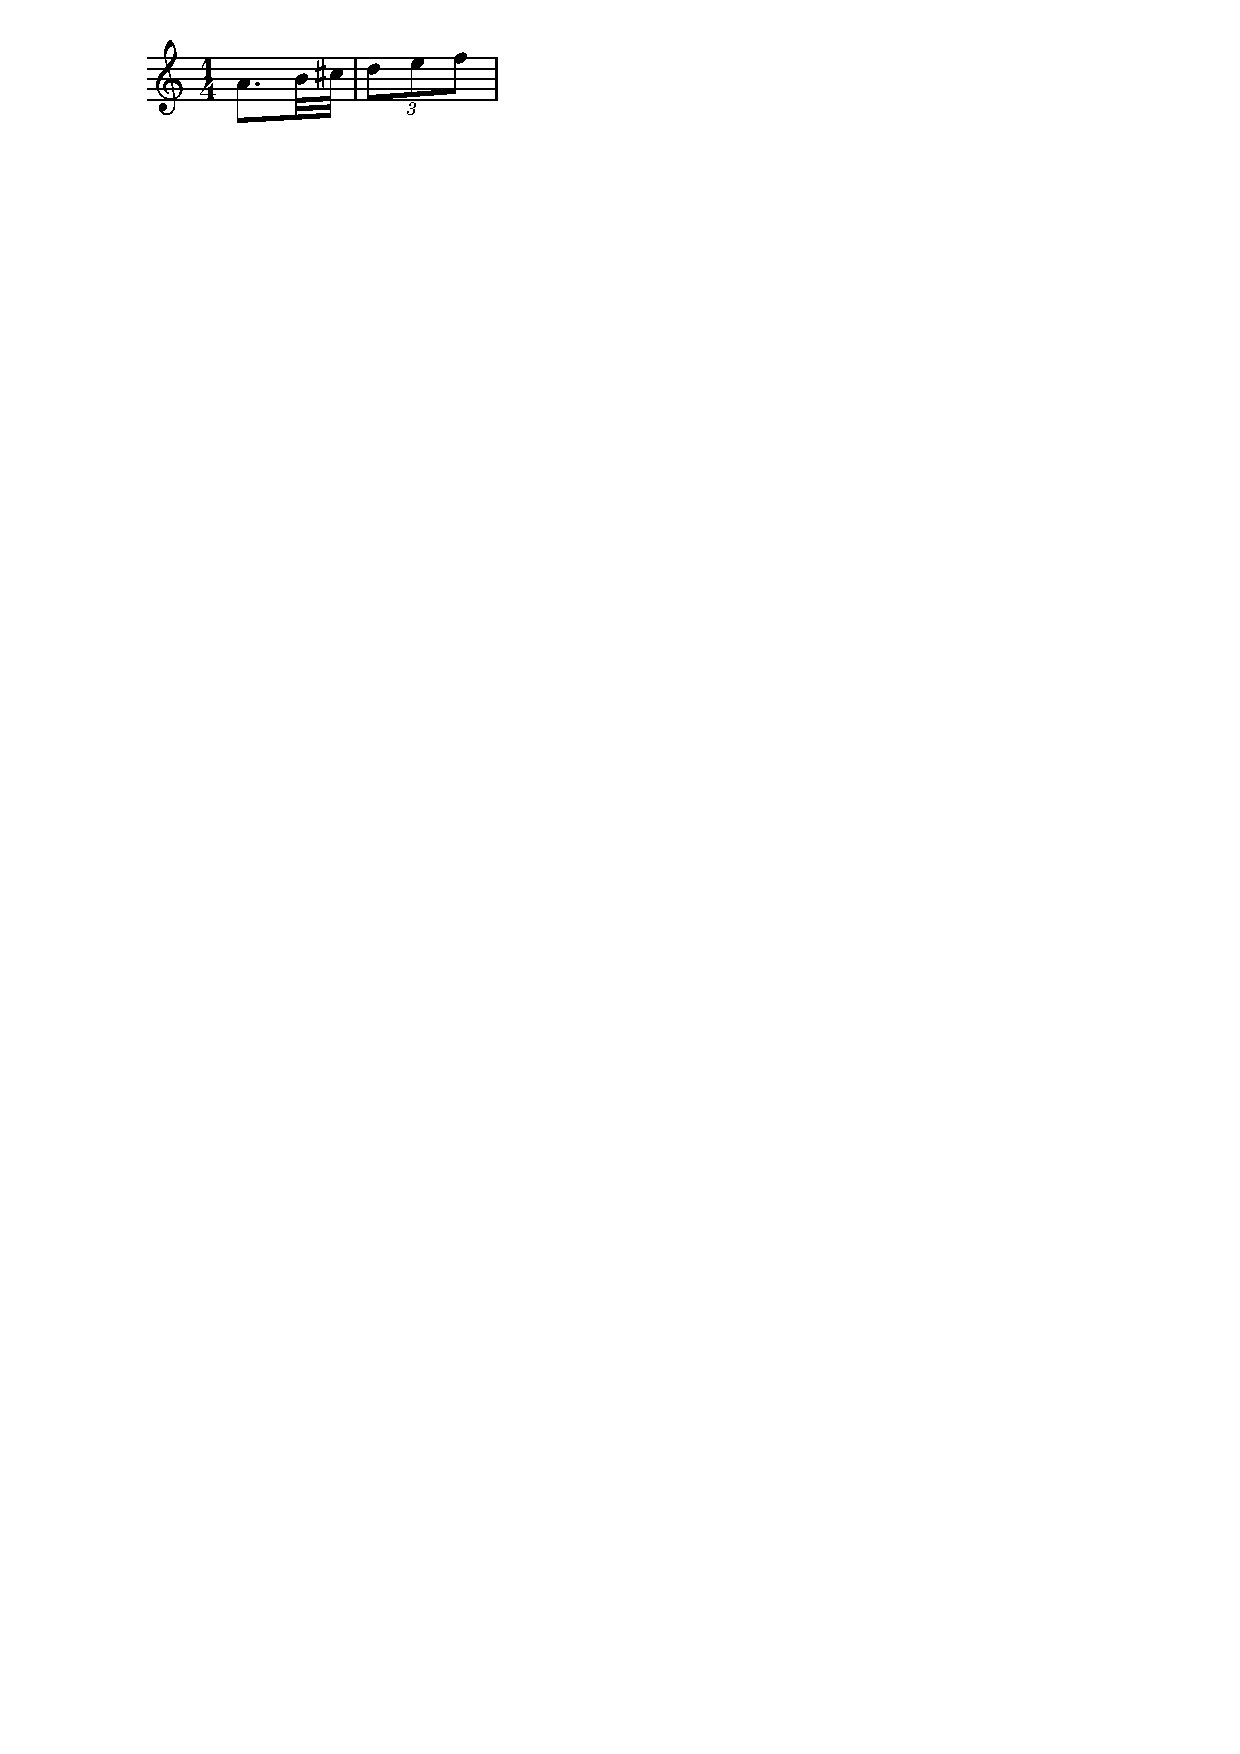
\includegraphics[scale=0.35,trim=0 5mm 0 0]{pictures/ex1.pdf},
  %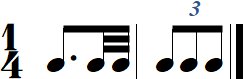
\includegraphics[scale=0.20]{pictures/score5.png},
corresponds to a hierarchical structure
that can be linearized as the sequence
$O =$
$\ccall{\mathsf{m}}\tstamp{[0,1]}$,
$\ccall{2}\tstamp{[0,1]}$,
$\mbox{\footnotesize A4}\tstamp{0}$,
$\ccall{2}\tstamp{[\frac{1}{2},1]}$,
$-\tstamp{\frac{1}{2}}$,
$\ccall{2}\tstamp{[\frac{3}{4},1]}$,
$\mbox{\footnotesize B4}\tstamp{\frac{3}{4}}$,
$\mbox{\footnotesize C$\sharp$5}\tstamp{\frac{7}{8}}$,
$\creturn{2}\tstamp{1}$,
$\creturn{2}\tstamp{1}$,
$\creturn{2}\tstamp{1}$,
$\creturn{\mathsf{m}}\tstamp{1}$,
$\ccall{\mathsf{m}}\tstamp{[1,2]}$,
$\ccall{3}\tstamp{[1,2]}$,
$\mbox{\footnotesize D5}\tstamp{1}$,
$\mbox{\footnotesize E5}\tstamp{\frac{4}{3}}$,
$\mbox{\footnotesize F5}\tstamp{\frac{5}{3}}$,
$\creturn{3}\tstamp{2}$,
$\creturn{\mathsf{m}}\tstamp{2}$.
%\end{enumerate}
The opening markups $\ccall{\mathsf{m}}$ %and $\creturn{\mathsf{m}}$
delimit \emph{measures},
which are time intervals of duration~1 in this example,
while the subsequences of $O$ between markups~$\ccall{d}$ and~$\creturn{d}$,
for some natural number~$d$,
represent a division of the time interval attached to $\ccall{d}$,
of duration $\ell$,
into $d$ sub-intervals of equal duration $\frac{\ell}{d}$.
%
We will show that $O$ is a solution for the
parsing of $I$. Note that several other parsings are possible
like \eg 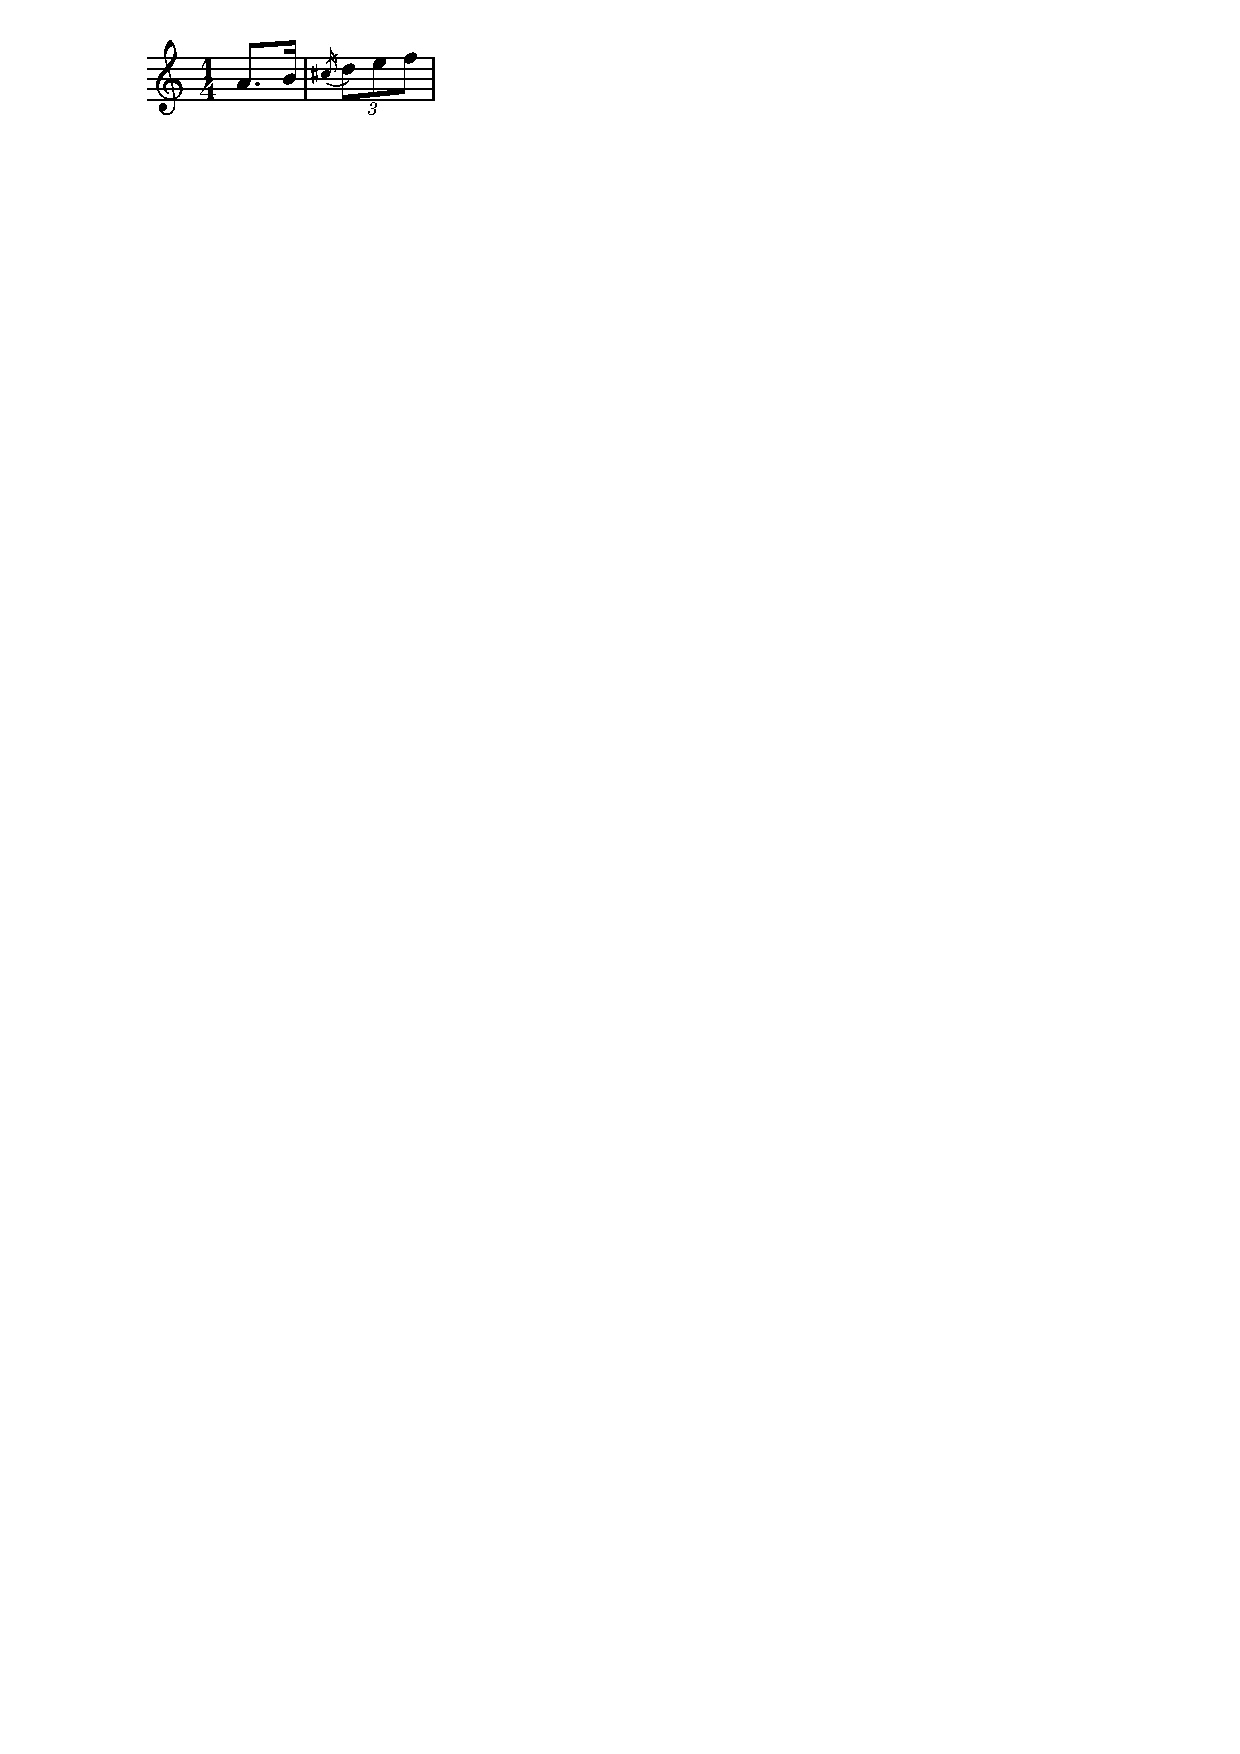
\includegraphics[scale=0.35,trim=0 5mm 0 0]{pictures/ex2.pdf}.
SW-parsing associates a weight value
to each solution, and our approach
aims at selecting the best one with respect to this weight.
\endex
\end{example}
